\section{Evaluation}
\label{sec:evaluation}

% \textcolor{red}{Maybe we can draw a plot here to show different meta axes. }
% How do you make the evaluation part reflect inference-time trustworthiness, not just generic trustworthiness?

% (1) group by how inference-time methods are evaluated,
% e.g. behavioral metrics (refusal accuracy for guardrails, response consistency for multi-agent)

% Hightlight the uniqueness of the evaluation dimension in inference-time methods (clear definition on each metrics and why they are importance to this paper)

Inference-time trustworthiness methods intervene after model training to shape LLM behavior under deployment constraints. As these interventions differ a lot in where and how they act, such as in prompts, logits, activations, external filters, or the system workflow, evaluation cannot be unified by one benchmark or one metric family. We therefore adopt a meta-axis evaluation view on the inference-time evaluation. The goal is to capture deployment-relevant properties that arise specifically from runtime trustworthiness. In practice, such enforcement is shaped by latency, cost, and integration constraints. Each axis highlights a distinct evaluation question, and while the axes are conceptually unique, they can overlap in practice:

\begin{figure*}[htbp]
  \centering
  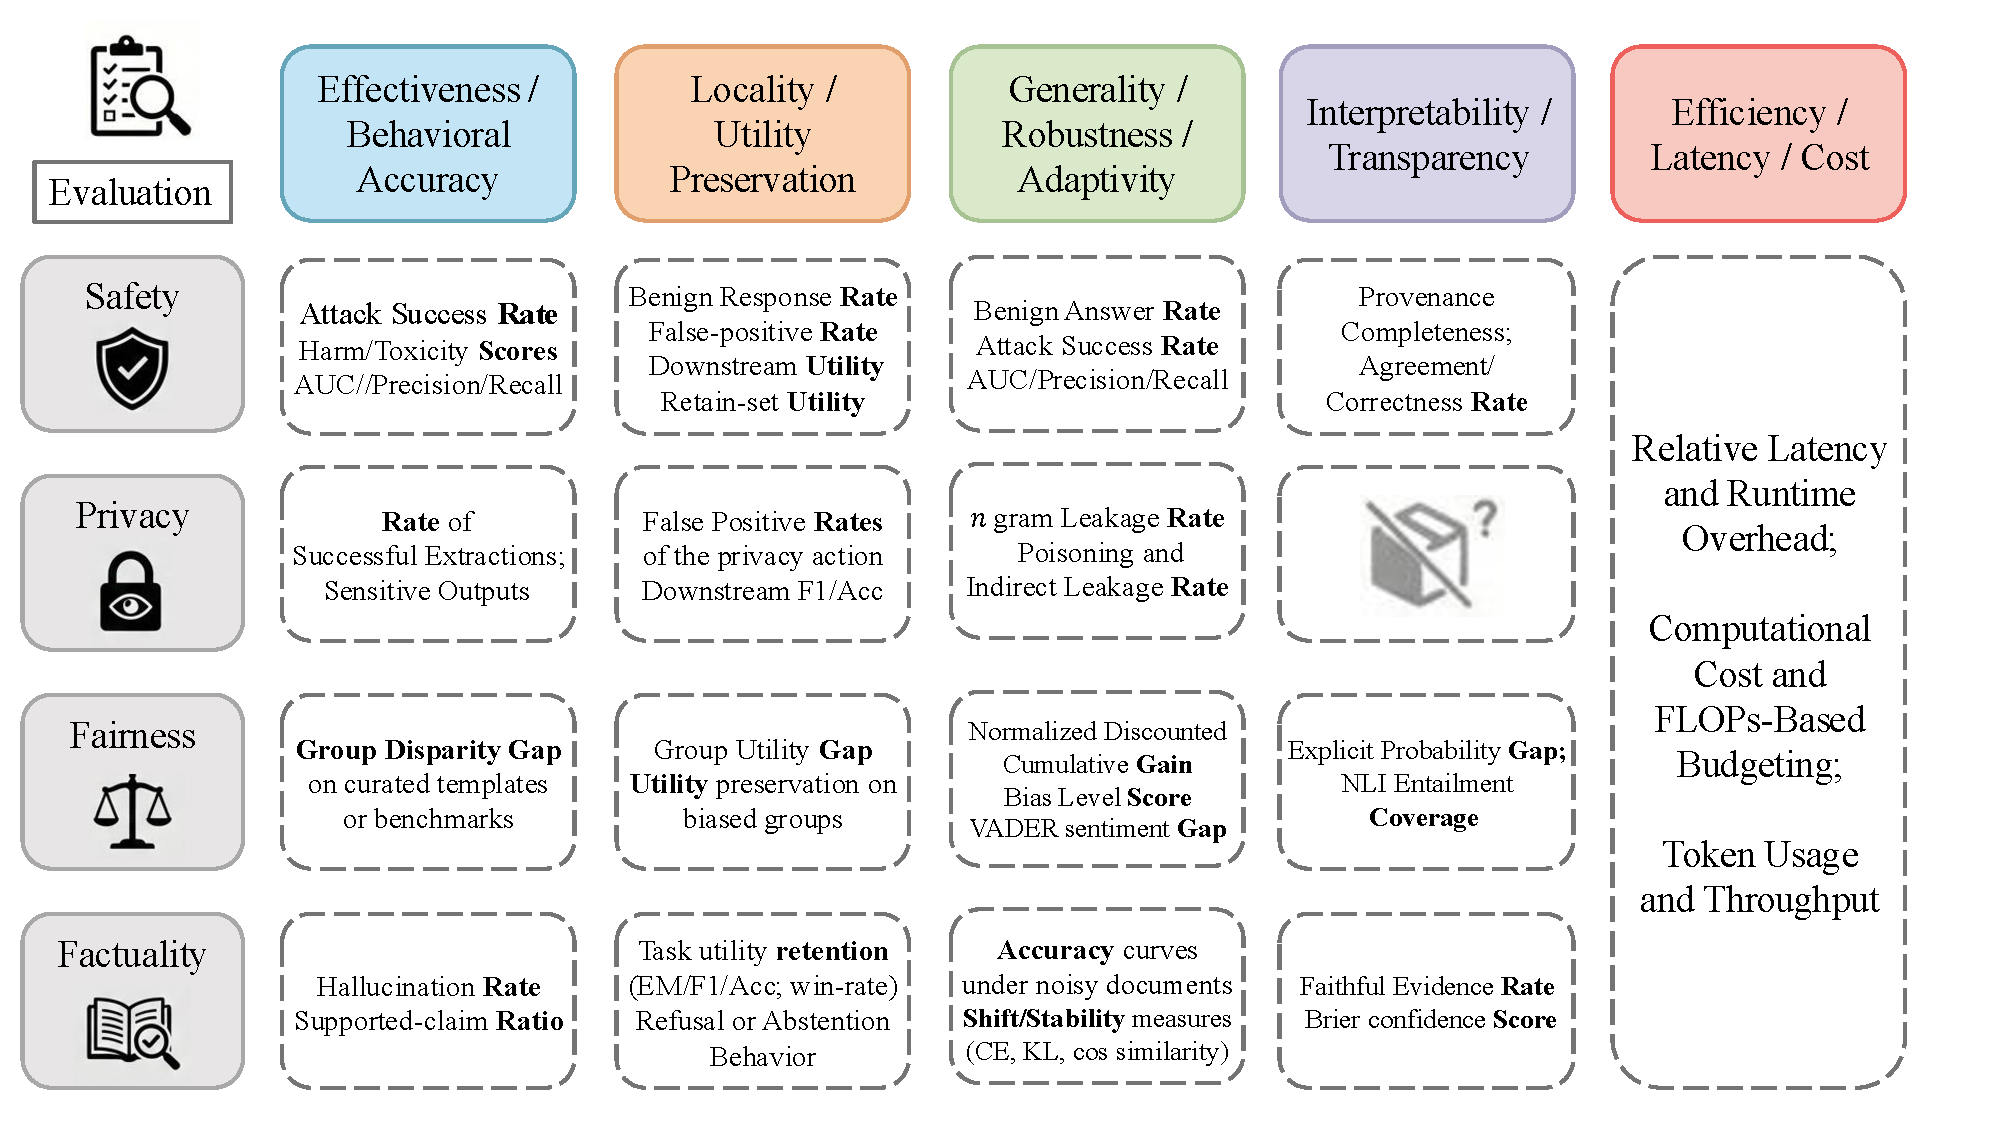
\includegraphics[width=1\linewidth]{figures/method/evaluations.pdf}
  \caption{\textcolor{red}{TODO: Evaluations}}
  \label{fig:evaluation}
\end{figure*}

\begin{itemize}
\item \textbf{Effectiveness / Behavioral Accuracy}: To what extent does the inference-time mechanism reliably enforce the intended behavioral constraints, and under what conditions does it fail?
\item \textbf{Locality / Utility Preservation}: To what extent are the intervention effects localized to the targeted behaviors while preserving general task performance and user utility?
\item \textbf{Generality / Robustness / Adaptivity}: How well does the mechanism generalize across tasks, domains, and input distributions, and how robust is it to distributional shifts?
\item \textbf{Efficiency / Latency / Cost}: What additional runtime overhead does the mechanism introduce in terms of latency, compute, memory, or token usage?
\item \textbf{Interpretability / Transparency}: To what extent are the mechanism’s actions, triggers, and decision rationales transparent to human auditors or downstream systems?
\end{itemize}

Although these axes separate different deployment concerns, they often trade off against one another. 
% For example, a guardrail detector may score highly on effectiveness, such as achieving a high AUC, yet still fail on locality by excessively blocking benign content. Similarly, a method can succeed on safety under standard conditions but fail on robustness when it is bypassed by prompt injection.
Building on this framing, this section organizes evaluation along the axes above and surveys representative metrics, across four categories: Safety, Privacy, Fairness, and Factuality.

\subsection{Effectiveness / Behavioral Accuracy}
Effectiveness / Behavioral Accuracy evaluates whether an inference-time mechanism $\mathcal{M}$ changes model behavior in the intended direction on a target evaluation distribution. Consider an LLM that produces an output $Y_{\mathcal{M}}(x)$ for an input $x \sim \mathcal{D}$ under $\mathcal{M}$. Effectiveness asks whether $\mathcal{M}$ increases the likelihood of desired trust-aligned behavior and decreases the likelihood of undesired behavior:
\[
\text{Effectiveness}(\mathcal{M}) \propto
\mathbb{E}_{x \sim \mathcal{D}}
\Big[
\mathbf{1}\{Y_{\mathcal{M}}(x)\in \mathcal{Y}_{\text{desired}}\}
-
\mathbf{1}\{Y_{\mathcal{M}}(x)\in \mathcal{Y}_{\text{undesired}}\}
\Big].
\]
In inference-time settings, this axis primarily measures the runtime behavior induced by a plug-in control layer, such as refusal, redaction, constrained decoding, evidence grounding, or verification. However, Effectiveness alone does not tell whether improvements come from overly broad suppression of benign behavior, from brittle operating thresholds, or from masking the underlying capability. These trade-offs motivate complementary axes such as Locality (utility and over-refusal), Robustness (bypassability and shift), Efficiency (latency/cost), and Interpretability (auditability).


% Effectiveness / Behavioral Accuracy evaluates the extent to which an inference-time mechanism $\mathcal{M}$ enforces the intended behavioral constraints on the target evaluation distribution, and characterizes when it does not. Consider an LLM (or an LLM-based system) that produces an output $Y_{\mathcal{M}}(x)$ for an input $x \sim \mathcal{D}$ under $\mathcal{M}$. Effectiveness asks whether $\mathcal{M}$ increases the likelihood of desired trust-aligned behavior and decreases the likelihood of undesired behavior:
% \[
% \text{Effectiveness}(\mathcal{M}) \propto
% \mathbb{E}_{x \sim \mathcal{D}}
% \left[
% \mathbf{1}\!\left\{Y_{\mathcal{M}}(x)\in \mathcal{Y}_{\text{desired}}\right\}
% -
% \mathbf{1}\!\left\{Y_{\mathcal{M}}(x)\in \mathcal{Y}_{\text{undesired}}\right\}
% \right].
% \]
% In practice, Effectiveness is measured using task-specific or risk-specific metrics that align with the intended trust objective, and it is often reported together with a breakdown by input type, threat model, or operating point. Effectiveness does not capture side effects on benign behavior, performance under distribution shift, runtime overhead, or auditability. These aspects are evaluated under separate axes, including Locality, Robustness, Efficiency, and Interpretability.


\subsubsection{Safety} 

Safety effectiveness measures whether a system suppresses harmful behavior at inference time when facing adversarial or high-risk prompts. In our taxonomy, the most common safety metrics are rate-based metrics that quantify how often unsafe behavior still occurs during deployment. This family includes attack-success-rate-style metrics such as jailbreak success rate, unsafe completion rate, and the complementary defense success rate. It also includes risk-score-based formulations that measure the proportion of outputs whose toxicity or harm score exceeds a threshold. From a unified perspective, both types of metrics quantify how often the system produces unsafe behavior at inference time. They differ mainly in whether safety is determined by a discrete attack outcome or by a continuous risk signal. Such metrics are widely used across context engineering \citep{kumar2024certifying, cao2024defending, ji2024defending, zhou2024defending}, guardrails \citep{DBLP:journals/corr/abs-2504-00441, DBLP:conf/nips/HanREJL00D24, sharma2025constitutional, Padhi2024GraniteG, Lees2022ANG, Zeng2025ShieldGemma2R}, decoding \citep{Xu2024SafeDecodingDA, Liu2024AlignmentEnhancedDD, Zeng2024RootDS, Zhao2024AdversarialCD, Huang2024SafeAlignerSA, Gallego2025MetaSCTS, Ghosal2024ImmuneIS}, representation engineering \citep{Arditi2024SingleDirection, Lee2024CAST, Sheng2025AlphaSteer, zhao2025adasteer}, pruning \citep{hasan2024pruning, chen2025safeptr, li-etal-2025-hierarchical, zhao2025understanding, DBLP:conf/emnlp/XuG0BS24, DBLP:conf/icml/HongDZLXLDBJXKH24, zhang2025activation}, unlearning \citep{deng2025guard, yan2025dual, zhang2024theft, DBLP:conf/acl/TakashiroKGCIM25}, and multi-agent defenses \citep{asad2025reddebatesaferresponsesmultiagent, fan2025peerguarddefendingmultiagentsystems, qi2025amplifiedvulnerabilitiesstructuredjailbreak, DBLP:conf/acl/HeLD00025, DBLP:conf/acl/Shahroz0YF025}. When an explicit guardrail is used, standard classification metrics such as AUC, AUPRC, Precision, Recall, and F1 are often also reported \citep{Padhi2024GraniteG, Chi2024LlamaG3, Zeng2025ShieldGemma2R, Kumar2025PolyGuardAM, Lee2025SafeRouteAM, Liu2025GuardReasonerTR}. 

These metrics are essential because they directly reflect whether harmful outputs still appear during inference time. However, a low unsafe rate does not necessarily imply a safer system, since it may result from an overly conservative operating point that also blocks benign requests. In inference-time settings, this issue is especially important because outcomes can depend heavily on threshold calibration, judge choice, and detector sensitivity, while adaptive attackers may evade methods through paraphrasing or prompting. For this reason, safety effectiveness should be evaluated together with Locality, Robustness, and Interpretability.


% The effectiveness on safety is commonly evaluated by whether the system refuses or blocks harmful outputs when facing adversarial or high-risk prompts. Among the metrics in our taxonomy, the most frequently used metric for safety effectiveness is the \emph{attack success rate} family:
% \[
% \mathrm{ASR}
% =
% \frac{\#\{\text{harmful responses}\}}
% {\#\{\text{attack prompts}\}}.
% \]
% Common variants include \emph{jailbreak success rate} (JSR), \emph{unsafe completion rate}, and the complementary \emph{defense success rate} $1-\mathrm{ASR}$. ASR family appears across a wide range of inference-time approaches, including context engineering \citep{kumar2024certifying, cao2024defending, ji2024defending, zhou2024defending}, guardrails \citep{DBLP:journals/corr/abs-2504-00441, DBLP:conf/nips/HanREJL00D24, sharma2025constitutional}, decoding \citep{Xu2024SafeDecodingDA, Liu2024AlignmentEnhancedDD, Zeng2024RootDS, Zhao2024AdversarialCD, Huang2024SafeAlignerSA, Gallego2025MetaSCTS, Ghosal2024ImmuneIS}, representation engineering \citep{Arditi2024SingleDirection, Lee2024CAST, Sheng2025AlphaSteer, zhao2025adasteer}, pruning \citep{hasan2024pruning, chen2025safeptr, li-etal-2025-hierarchical, zhao2025understanding}, unlearning \citep{deng2025guard, yan2025dual, zhang2024theft, DBLP:conf/acl/TakashiroKGCIM25}, and multi-agent defenses \citep{asad2025reddebatesaferresponsesmultiagent, fan2025peerguarddefendingmultiagentsystems, qi2025amplifiedvulnerabilitiesstructuredjailbreak, DBLP:conf/acl/HeLD00025, DBLP:conf/acl/Shahroz0YF025}. ASR is widely used because it directly measures whether harmful behavior still occurs during inference. However, a low ASR may reflect an operating point that also rejects many benign requests. For this reason, safety effectiveness should be interpreted together with Locality metrics that quantify benign pass rate and task utility under safe prompts, and with Robustness metrics that test transfer across jailbreak sets, multi-turn settings, and different judge models.

% A closely related family uses scalar harm or toxicity scores $\mathrm{Risk}(Y)$ to report mean risk or the fraction of outputs above a threshold $\tau$:
% \[
% \mathrm{UnsafeRate}
% =
% \frac{\#\{Y : \mathrm{Risk}(Y)>\tau\}}{\#\{\text{outputs}\}}.
% \]
% This formulation is widely used in guardrails \citep{Padhi2024GraniteG, Lees2022ANG, Zeng2025ShieldGemma2R} and editing \citep{wang2024detoxifying, uppaal2024model} settings. It also appears in compression or pruning studies \citep{DBLP:conf/emnlp/XuG0BS24, DBLP:conf/icml/HongDZLXLDBJXKH24, zhang2025activation}, where the goal is to test whether efficiency-oriented interventions degrade safety-related behavior. However, in inference-time deployment, the choice of risk model and threshold becomes particularly consequential. Small differences in calibration can change whether an output is blocked or allowed. Moreover, adaptive attackers may evade detectors through paraphrasing or multi-step prompting. Accordingly, Robustness evaluations under adaptive attacks and distribution shift, as well as Interpretability for policy-auditable decisions, are often needed to contextualize these scores. When the mechanism includes a guardrail, standard classification metrics (AUC/AUPRC/Precision/Recall/F1) are also reported \citep{Padhi2024GraniteG, Chi2024LlamaG3, Zeng2025ShieldGemma2R, Kumar2025PolyGuardAM, Lee2025SafeRouteAM, Liu2025GuardReasonerTR}, but strong detector metrics do not necessarily translate to better end-to-end safety without a well-chosen operating point.

% For guardrail-based approaches, safety effectiveness is often formulated as a classification problem, such as harmful content detection, jailbreak detection, or prompt injection detection. Thus, evaluation uses standard classification metrics, including AUC, AUPRC, and Precision, Recall, and F1 \citep{Padhi2024GraniteG, Chi2024LlamaG3, Zeng2025ShieldGemma2R, Kumar2025PolyGuardAM, Lee2025SafeRouteAM, Liu2025GuardReasonerTR}. This family is applied when the inference-time mechanism is itself a detector, or when it includes a detector as part of a pipeline. In practice, strong classifier performance does not necessarily imply better safety effectiveness, because the operating threshold and calibration can dominate system behavior, and real-world inputs often differ substantially from the evaluation distribution.

% \subsubsection{Privacy}

% Privacy effectiveness evaluates whether an inference-time mechanism reduces the model's tendency to reveal sensitive information, including memorized training content, personally identifying information (PII), or private passages surfaced through retrieval. A dominant family measures memorization or extraction success, which is similar to the ASR family. It counts how often an attacker can recover sensitive spans or training text \citep{pawelczyk2023context, DBLP:conf/inlg/IppolitoTNZJLCC23, Borec2024TheUI, yan2025dual}.  A common metric is the extraction success rate:
% \[
% \mathrm{ExtractSR}
% =
% \frac{\#\{\text{successful extractions}\}}
% {\#\{\text{extraction attempts}\}},
% \]
% where ``success'' can be defined by exact match, near-verbatim overlap, or a task-specific leakage rule. This family is widely used because it directly evaluates whether an attacker can still elicit memorized content. Another similar variant is to measure how often sensitive content appears in the final output. A simple form is the \emph{disclosure rate}:
% \[
% \mathrm{DisclosureRate}
% =
% \frac{\#\{\text{sensitive output spans}\}}
% {\#\{\text{outputs}\}}.
% \]
% This variant is commonly used in privacy-focused decoding and retrieval controls that filter or constrain generation to avoid exposing sensitive retrieved data \citep{Wang2025PrivacyAwareDM, Ok2024DecodingWL, Wei2024PrivacyRO, zou2025poisonedrag}. Yet these metrics depend strongly on the attack design and on how the overlap is defined. Thus, automated detectors can miss paraphrased leakage while over-flagging benign overlaps, and cross-language transfer of leakage detection is often weak.

% Another widely used family is to evaluate privacy effectiveness through the success of membership inference, often measured by attack accuracy or AUC \citep{zou2025poisonedrag, nakka2025piijailbreaking}. Successful defenses reduce the attack's advantage toward random guessing. Relatedly, in-context unlearning work frames privacy protection as removing the influence of selected in-context examples or documents at inference time, and evaluates effectiveness by the change in predictions attributable to the removed context \citep{pawelczyk2023context, muresanufast, liu2024learning}. These evaluations also have weaknesses. Membership and property inference depend on assumptions about the adversary's access and auxiliary knowledge. In unlearning evaluations, observed behavioral changes may reflect refusal or suppression rather than genuine forgetting. A model can decline to answer while the private information remains encoded in its parameters. It is still challenging to verify actual removal, as opposed to surface-level avoidance.


\subsubsection{Privacy}
% Privacy effectiveness evaluates whether an inference-time mechanism reduces leakage of sensitive information, including memorized training text, personally identifying information (PII), or private passages surfaced through retrieval. A dominant family measures extraction or memorization success:
% \[
% \mathrm{ExtractSR}
% =
% \frac{\#\{\text{successful extractions}\}}
% {\#\{\text{extraction attempts}\}},
% \qquad
% \mathrm{DisclosureRate}
% =
% \frac{\#\{\text{sensitive output spans}\}}
% {\#\{\text{outputs}\}}.
% \]
% ExtractSR counts how often an attacker can recover sensitive spans or training text \citep{pawelczyk2023context, DBLP:conf/inlg/IppolitoTNZJLCC23, Borec2024TheUI, yan2025dual}. DisclosureRate is commonly used in privacy-focused decoding and retrieval controls that filter or constrain generation to avoid exposing sensitive retrieved data \citep{Wang2025PrivacyAwareDM, Ok2024DecodingWL, Wei2024PrivacyRO, zou2025poisonedrag}. In inference-time settings, however, many privacy defenses act through redaction or refusal at the output level. This creates a mode of hiding information rather than forgetting, which can lead to a failure mode of hiding rather than forgetting. Leakage detection is also fragile to paraphrase, indirect disclosure, and cross-language variation, so Robustness tests with stronger extraction strategies and broader leakage definitions are important. Membership inference success (attack accuracy/AUC) is sometimes used as well \citep{zou2025poisonedrag, nakka2025piijailbreaking}, but it remains sensitive to assumptions about the adversary's access and auxiliary knowledge, and should be reported with clear threat models.
Privacy effectiveness evaluates whether an inference-time method reduces leakage of sensitive information, such as memorized training text, personally identifying information, or private content. The most common metrics measure how often sensitive information can still be extracted or disclosed, for example through extraction success rate or disclosure rate. The former captures whether an attacker can recover sensitive spans or memorized text \citep{pawelczyk2023context, DBLP:conf/inlg/IppolitoTNZJLCC23, Borec2024TheUI, yan2025dual}. The latter is common in privacy-oriented decoding and retrieval controls, where the goal is to reduce the fraction of outputs that contain sensitive content \citep{Wang2025PrivacyAwareDM, Ok2024DecodingWL, Wei2024PrivacyRO, zou2025poisonedrag}. However, many inference-time privacy defenses work mainly through output-level refusal or redaction. As a result, they often hide information rather than remove the underlying memory. This makes Robustness especially important, since leakage detection can be brittle to paraphrase, indirect disclosure, and cross-lingual variation. Some work also reports membership inference accuracy or AUC \citep{zou2025poisonedrag, nakka2025piijailbreaking}, but these metrics depend strongly on the assumed threat model and auxiliary knowledge.

\subsubsection{Fairness}
% Fairness effectiveness evaluates whether an inference-time mechanism reduces biased behavior in outputs, such as stereotypes, unequal toxicity across demographic groups, or skewed recommendations. Compared to safety, fairness evaluation is more task-specific, but several metric families appear frequently. A common approach is to measure bias scores on curated templates or benchmarks, such as how often the model associates certain roles with a protected group, or how it responds to prompts involving sexual identity or other sensitive attributes. Prompting- and context-based interventions report reductions in these bias scores after applying fairness-aware prompts or in-context demonstrations \citep{dwivedi2023breaking, huang2024bias, fayyazi2025facter, dhingra2023queer, kamruzzaman2024prompting}. These scores are widely used because they directly target the intended fairness behavior. This family has clear limitations. Bias scores are often tied to a small set of templates and attributes, so improvements may not generalize to richer inputs or to intersectional groups. Template-based tests can emphasize shallow patterns of bias and miss more subtle stylistic or pragmatic forms. In addition, fairness scores can be sensitive to the evaluation prompt format, making it hard to compare numbers across papers.

% Another widely used family measures the \emph{disparity} of an outcome metric across groups. Given a metric $m(\cdot)$ (e.g., toxicity score, error rate, refusal rate), a simple group gap is:
% \[
% \Delta_{\mathrm{group}}
% =
% \left|\, \mathbb{E}[m(Y)\mid g{=}a] \;-\; \mathbb{E}[m(Y)\mid g{=}b] \,\right|.
% \]
% Fairness-aware context engineering uses similar ideas to evaluate whether retrieved evidence and downstream outputs become more balanced across groups \citep{chen2024spica, shrestha2024fairrag}. Editing and pruning methods also report disparity reductions when they target bias-related structure inside the model \citep{cai2024locating, qin2024mitigating, zayed2024fairness, dasu2025attention, ma2025breaking}. However, this family requires explicit group definitions and labels, which may be unavailable or sensitive. It also does not automatically imply fairness in a broader sense, since group parity can be achieved by degrading performance for everyone. Because of this, fairness effectiveness should be read together with locality and utility metrics.
Fairness effectiveness evaluates whether an inference-time mechanism reduces biased behavior, such as stereotypes, uneven toxicity across demographic groups, or skewed recommendations. Common evaluations include bias scores on curated templates or benchmarks \citep{dwivedi2023breaking, huang2024bias, fayyazi2025facter, dhingra2023queer, kamruzzaman2024prompting} and group disparity gaps. Given an outcome metric $m(\cdot)$ (e.g., toxicity, error rate, refusal rate), a simple group gap is:
\[
\Delta_{\mathrm{group}}
=
\left|\, \mathbb{E}[m(Y)\mid g{=}a] \;-\; \mathbb{E}[m(Y)\mid g{=}b] \,\right|.
\]
Fairness-aware context engineering uses similar ideas to evaluate whether retrieved evidence and downstream outputs become more balanced across groups \citep{chen2024spica, shrestha2024fairrag}. Editing and pruning methods also report disparity reductions when they target bias-related structure inside the model \citep{cai2024locating, qin2024mitigating, zayed2024fairness, dasu2025attention, ma2025breaking}. These metrics can directly reflect the intended fairness behavior, especially for prompt- and context-based interventions. In inference-time systems, however, parity can be improved by raising refusal or by making responses more uniform in style, rather than by improving equitable helpfulness. Thus, fairness effectiveness should be considered with Locality metrics that report per-group utility and over-refusal. Template-based bias scores are also sensitive to prompt form and may not generalize to richer inputs or intersectional groups, motivating Robustness evaluations across formats, domains, and languages. For deployment, Interpretability is often needed because fairness policies may require transparent, auditable decision rules.




\subsubsection{Factuality}
% Factuality effectiveness evaluates whether an inference-time mechanism reduces hallucinations and increases factual correctness or groundedness. A common formulation treats hallucinations as errors and reports a hallucination rate:
% \[
% \mathrm{HallucRate}
% =
% \frac{\#\{\text{unsupported or incorrect outputs}\}}
% {\#\{\text{evaluated outputs}\}}.
% \]
% Prompting and self-correction methods report hallucination reductions using verification or reflection routines \citep{dhuliawala2024chain, li2024think, feng2024teaching}. In multimodal settings, decoding-time methods evaluate hallucination with respect to the input image or video and report reduced hallucinated content under contrastive or penalty decoding \citep{Park2024ConVisCD, Yuan2024HELPDMH, Suo2025OctopusAH}. Nevertheless, hallucination labels are often noisy, and automatic detectors can be uncalibrated or biased. Many tasks have multiple valid answers, so binary hallucination labels can be too strict. Results are also sensitive to prompt format and judging protocol, which complicates direct comparisons across papers.

% Another common family is task accuracy (e.g., EM/F1/Acc on QA) or truthfulness scores on benchmarks. Representation engineering methods report improved truthfulness by steering internal activations, often measured by benchmark accuracy gains \citep{li2023iti, bayat2024enhanced, wang2024act, liu2024uth, li2025truthneurons}. Editing methods evaluate effectiveness via edit success on targeted facts and improved correctness on edited queries \citep{meng2022locating, meng2022memit, hartvigsen2024aging, wang2024wise}. These metrics also have weaknesses. Accuracy gains may come from conservative behavior rather than better factual knowledge, especially when the mechanism encourages refusal under uncertainty. Benchmark improvements can overestimate real-world factual reliability because benchmarks are static and limited in coverage. In addition, improvements on one domain can fail on new domains or long-form generation, which should be assessed under robustness.

% In Context Engineering settings, factuality is often evaluated through whether the answer is supported by the provided evidence. A simple form is the supported-claim ratio:
% \[
% \mathrm{GroundedRate}
% =
% \frac{\#\{\text{claims supported by evidence}\}}
% {\#\{\text{all claims}\}}.
% \]
% Many works implement groundedness as a detection task and report AUC/AUPRC/F1 for identifying unsupported claims or hallucination risk \citep{asai2024self, zhou2024metacognitive}. Groundedness metrics are valuable because they tie factuality to explicit evidence, yet they have weaknesses. They depend largely on retrieval coverage and corpus quality. If evidence is missing, groundedness metrics can conflate retrieval failure with generation failure.

Factuality effectiveness evaluates whether an inference-time mechanism reduces hallucinations and improves factual correctness or groundedness. A common formulation treats hallucinations as errors and reports a hallucination rate:
\[
\mathrm{HallucRate}
=
\frac{\#\{\text{unsupported or incorrect outputs}\}}
{\#\{\text{evaluated outputs}\}}.
\]
Prompting and self-correction methods report hallucination reductions using verification or reflection routines \citep{dhuliawala2024chain, li2024think, feng2024teaching}, with similar practices also appearing in multimodal settings \citep{Park2024ConVisCD, Yuan2024HELPDMH, Suo2025OctopusAH}. Task accuracy (EM/F1/Acc) and truthfulness scores on benchmarks are also widely used. Representation engineering steers internal activations to improve factuality, typically evaluated by benchmark accuracy \citep{li2023iti, bayat2024enhanced, wang2024act, liu2024uth, li2025truthneurons}. 
Similarly, editing is evaluated by edit success on targeted facts and accuracy on edited queries \citep{meng2022locating, meng2022memit, hartvigsen2024aging, wang2024wise}. Task accuracy is convenient and comparable, but for inference-time interventions it can be confounded by response format changes and by benchmark limitness. Therefore, accuracy should be paired with consistent prompting and answer-format constraints, and ideally stratified by question type to reveal where the mechanism actually improves correctness.


In context-based settings, groundedness is often evaluated by whether claims are supported by provided evidence. A simple supported-claim ratio is:
\[
\mathrm{GroundedRate}
=
\frac{\#\{\text{claims supported by evidence}\}}
{\#\{\text{all claims}\}}.
\]
Many works implement groundedness as a detection task and report AUC/AUPRC/F1 for identifying unsupported claims or hallucination risk \citep{asai2024self, zhou2024metacognitive}. Groundedness metrics align well with inference-time mechanisms that insert, filter, or re-rank evidence, because they evaluate the intended behavioral change. Yet they can blur retrieval and generation errors when evidence coverage is incomplete, and they are sensitive to the claim extraction and judging procedure. Consequently, factuality effectiveness in inference-time systems usually needs to be reported together with retrieval quality, and verified with robustness tests under perturbed or missing evidence.


\subsection{Locality / Utility Preservation}
Locality / Utility Preservation evaluates whether an inference-time mechanism $\mathcal{M}$ confines its behavioral changes to the intended scope while preserving user utility. Unlike training-time alignment, inference-time controls are typically implemented as plug-in layers. As a result, the dominant locality failure mode is behavioral spillover, in which the system becomes safer by being less helpful, issuing more refusals, or providing less information about requests that should have been served. Formally, let $\mathcal{D}_{\text{tgt}}$ denote the targeted distribution (e.g., harmful, sensitive, or bias-triggering prompts) and $\mathcal{D}_{\text{benign}}$ denote benign traffic. A generic utility retention view is:
\[
\Delta U_{\text{benign}}(\mathcal{M})
=
\mathbb{E}_{x\sim \mathcal{D}_{\text{benign}}}\!\left[u\!\left(Y_{\mathcal{M}}(x)\right) - u\!\left(Y(x)\right)\right],
\]
where $u(\cdot)$ can be task accuracy (EM/F1/Acc), LLM-as-judge helpfulness, or win-rate. In inference-time deployment, locality is coupled to thresholding and pipeline composition. When multiple strategies are combined, such as guardrails, decoding, and editing, they can amplify suppression of benign outputs even if each component appears acceptable in isolation.


\subsubsection{Safety}
For safety, locality metrics quantify how much a defense reduces harmful behavior \emph{without} broadly degrading benign outputs. In context engineering, locality is often reported explicitly via benign response rate alongside ASR. The metric directly evaluates whether the runtime defense alters original behaviors on safe prompts rather than merely lowering ASR by refusing more \citep{kumar2024certifying, cao2024defending, ji2024defending, zhou2024defending}. In guardrail systems, locality is naturally expressed through false positives on clean inputs or precision at a chosen operating point, since the runtime action is a binary filter or router. Accordingly, many works report false-positive rates, benign blocking rates, and downstream utility after filtering or routing \citep{Padhi2024GraniteG, Lees2022ANG, Zeng2025ShieldGemma2R, Chi2024LlamaG3, Kumar2025PolyGuardAM, Lee2025SafeRouteAM, Liu2025GuardReasonerTR}. Decoding defenses and representation engineering additionally measure whether the intervention distorts normal generation trajectories (e.g., via MT-Bench/helpfulness reward, win-rate, or safe-prompt compliance), making locality a measure of how much the logit mechanism perturbs benign token probabilities \citep{Xu2024SafeDecodingDA, Liu2024AlignmentEnhancedDD, Zeng2024RootDS, Gallego2025MetaSCTS, Ghosal2024ImmuneIS, Arditi2024SingleDirection, Lee2024CAST, Sheng2025AlphaSteer, zhao2025adasteer}. For safety during pruning, unlearning, and model merging, locality is typically evaluated using the retain-set utility. Common methods include general-purpose benchmarks, MT-Bench, and instruction-following scores. The goal is to test whether inference-time modifications preserve utility while improving refusal behavior on undesired data \citep{hasan2024pruning, chen2025safeptr, li-etal-2025-hierarchical, zhao2025understanding, deng2025guard, yan2025dual, zhang2024theft, DBLP:conf/acl/TakashiroKGCIM25}. In multi-agent defenses, locality often appears as false alarms on clean inputs, such as the false positive rate for trigger or backdoor detection, because a monitoring agent can incorrectly flag benign interactions and suppress the entire workflow \citep{fan2025peerguarddefendingmultiagentsystems, asad2025reddebatesaferresponsesmultiagent}.Across these settings, an inference-time-specific concern is that safety can be achieved by encouraging over refusals. Therefore, low attack success should be interpreted together with preserved benign utility under the same deployment configuration.

\subsubsection{Privacy}
Privacy locality asks whether a runtime privacy control prevents leakage selectively while preserving normal completion and retrieval utility. Many inference-time privacy defenses operate through output-layer refusal or retrieval filtering. In this setting, locality emphasizes minimizing collateral damage on non-sensitive content rather than demonstrating forgetting. Accordingly, common locality evaluations include utility retention on benign tasks under privacy controls, and false positives of the privacy action, such as blocking harmless queries. Retain accuracy and benign-task performance are often used to show that reducing outputs of undesired data does not broadly degrade utility \citep{pawelczyk2023context, DBLP:conf/inlg/IppolitoTNZJLCC23, Borec2024TheUI, yan2025dual}. In decoding and context engineering, locality is often evaluated through retrieval and answer utility. Filtering or constraining generation to avoid sensitive content should not sharply reduce correctness on non-sensitive questions, so papers report downstream EM/F1/Acc or task success together with privacy rates \citep{Wang2025PrivacyAwareDM, Ok2024DecodingWL, Wei2024PrivacyRO, zou2025poisonedrag}. A distinctive inference-time failure mode in privacy is hiding rather than forgetting. Aggressive redaction or refusal can reduce measured leakage, while the underlying memorization may remain. Therefore, privacy locality should track benign utility and false positives, and be considered alongside robustness tests against paraphrase or multilingual leakage.


\subsubsection{Fairness}
Fairness locality evaluates whether inference-time bias mitigation improves outcomes without degrading helpfulness, specificity, or access unevenly across groups. A frequent locality failure mode is that the system becomes “fair” by being generic or by refusing more for certain groups. Thus, beyond template-based bias scores, locality is naturally measured by per-group utility retention and refusal disparity. Given a utility metric $u(\cdot)$ (task success, judge helpfulness, recommendation quality), a standard locality view is the group-wise utility gap under the intervention. Simple group gaps can be:
\[
\Delta_{\mathrm{util}}
=
\left|\mathbb{E}[u(Y_{\mathcal{M}})\mid g{=}a]-\mathbb{E}[u(Y_{\mathcal{M}})\mid g{=}b]\right|,
\]
\[
\Delta_{\mathrm{refuse}}
=
\left|\mathbb{E}[\mathrm{Refuse}(Y_{\mathcal{M}})\mid g{=}a]-\mathbb{E}[\mathrm{Refuse}(Y_{\mathcal{M}})\mid g{=}b]\right|.
\]
Context engineering methods can report reduced bias while also tracking whether benign utility is preserved across prompts and demographics \citep{dwivedi2023breaking, huang2024bias, fayyazi2025facter, dhingra2023queer, kamruzzaman2024prompting}. In retrieval-augmented fairness, locality also refers to whether the RAG pipeline continues to return relevant information and maintains utility while improving group balance \citep{chen2024spica, shrestha2024fairrag}. For editing and pruning methods, locality is often evaluated as utility preservation (e.g., code correctness or general benchmarks) to ensure bias reduction is not obtained by broadly damaging the model \citep{cai2024locating, qin2024mitigating, zayed2024fairness, dasu2025attention, ma2025breaking}. In inference-time deployment, these locality metrics are particularly important because fairness policies are often enforced via thresholds and post-training alignments, which can create group-dependent false positives and silently shift utility.

\subsubsection{Factuality}
For factuality, locality captures whether hallucination reduction is achieved without sacrificing answer completeness, informativeness, and performance on queries the model could already answer correctly. Many inference-time factuality methods (self-correction, verification loops, constrained generation, evidence grounding, activation steering, or post-editing) change how the model generates rather than what it knows. Thus, locality in factuality is often about avoiding excessive abstention, short answers, or overly cautious language. Accordingly, locality is commonly reported as task utility retention (EM/F1/Acc, win-rate, judge helpfulness) on benign factual QA while measuring hallucination reductions \citep{dhuliawala2024chain, li2024think, feng2024teaching, Park2024ConVisCD, Yuan2024HELPDMH, Suo2025OctopusAH}. For representation engineering, locality is reflected in whether truthfulness gains transfer without harming general capabilities, often tracked via benchmark accuracy and refusal/abstention behavior on answerable queries \citep{li2023iti, bayat2024enhanced, wang2024act, liu2024uth, li2025truthneurons}. For editing-style approaches, locality is evaluated as minimal side effects on non-edited facts and overall task accuracy, which becomes even more sensitive when edits are used as inference-time corrections or deployed as lightweight patches \citep{meng2022locating, meng2022memit, hartvigsen2024aging, wang2024wise}. In context engineering, locality also requires differentiating retrieval failures from generation failures. Improvements in groundedness metrics should be considered with utility and evidence coverage, otherwise the system may appear more factual simply by refusing or by narrowing outputs to what is explicitly retrieved \citep{asai2024self, zhou2024metacognitive}. Overall, factuality locality in inference-time settings is best interpreted as a \emph{selective correctness gain} rather than a global output shift, and should be reported with explicit utility measures under certain answer-format constraints.



\subsection{Generality / Robustness / Adaptivity}
Generality / Robustness / Adaptivity evaluate whether an inference time mechanism $\mathcal{M}$ keeps its intended effect when inputs, tasks, or attackers change at deployment. This axis is not about a single test set. It is about performance over a family of conditions, which is likely out-of-distribution. Let $\{\mathcal{D}_k\}_{k=1}^K$ be test distributions and let $s_k(\mathcal{M})$ be a score on $\mathcal{D}_k$. A common summary reports both the average and the worst case:
\[
s_{\mathrm{avg}}(\mathcal{M})=\frac{1}{K}\sum_{k=1}^K s_k(\mathcal{M}),
\qquad
s_{\min}(\mathcal{M})=\min_{k\in[K]} s_k(\mathcal{M}).
\]
In inference-time settings, $s_{\min}$ is often more critical for deployment because the system must handle rare but high-risk inputs.

\subsubsection{Safety}
For safety, robustness metrics test whether refusals and constraints persist under new jailbreak styles and adaptive prompts.
Many prompt and context methods report Attack Success Rate ($\mathrm{ASR}$) together with Benign Answering Rate ($\mathrm{BAR}$). This evaluates whether the safety behavior generalizes across multiple jailbreak distributions \citep{kumar2024certifying, cao2024defending, zhou2024defending}.
A robust summary can be written over attack families $\mathcal{A}$ as:
\[
\mathrm{ASR}_{\max}(\mathcal{M})
=
\max_{a\in\mathcal{A}} \mathrm{ASR}_a(\mathcal{M}),
\qquad
\mathrm{BAR}_{\min}(\mathcal{M})
=
\min_{a\in\mathcal{A}} \mathrm{BAR}_a(\mathcal{M}).
\]
Several studies also report $\Delta \mathrm{ASR}$ and $\Delta \mathrm{BAR}$ when the guard strength or policy changes.
This measures sensitivity to thresholds and operating points, which is central at inference time \citep{DBLP:journals/corr/abs-2504-00441}.

Decoding, representation engineering, and unlearning methods often evaluate robustness by running the same $\mathrm{ASR}$ under stronger or more diverse attacks while tracking judge-based safety scores. \citep{deng2025guard, yan2025dual}
Typical reported signals include Harmful Score and Safety Score on a fixed scale, with utility accuracy on task suites \citep{Xu2024SafeDecodingDA, Wang2024InferAligner, Gallego2025MetaSCTS}.
These metrics evaluate whether runtime control holds when the prompt is adversarial, while the utility performance stays unchanged. Pruning and model merging methods report \emph{Average ASR} across safety benchmarks and track restoration ratios \citep{li-etal-2025-hierarchical, djuhera2025safemerge, DBLP:journals/corr/abs-2412-19512}. Guardrails and multi-agents systems emphasize generality across domains and languages by reporting detector metrics such as precision, recall, F1, AUC, and AUPRC on multiple benchmarks \citep{Inan2023LlamaGL, Padhi2024GraniteG, Upadhayay2025XGuardMG, Ghosh2024AEGISOA, asad2025reddebatesaferresponsesmultiagent}.
Calibration is also reported with Expected Calibration Error $\mathrm{ECE}$.
This tests whether the same decision threshold remains reliable under shift \citep{DBLP:conf/iclr/0002HGWW25, DBLP:conf/acl/FengS00BT24}. At inference time, robustness is often achieved by stronger refusals or more aggressive rewrites.
This can lead to overrefusal, which can be observed through the BAR and over-defense rate \citep{cao2024defending, zhou2024defending}.
It can also lead to overcost, especially for guardrails and multi agent systems, because they add extra checks and additional model calls at inference time \citep{DBLP:conf/icml/LiGZFL25, Sharma2025ConstitutionalCD, lakara2025llmconsensusmultiagentdebatevisual, song2024auditllmmultiagentcollaborationlogbased}.


\subsubsection{Privacy}
For privacy, robustness metrics test whether the control of leakage still holds under different attacker models and different privacy budgets.
Inference time privacy mechanisms often target multiple inference attacks.
A common reporting pattern is $1-\mathrm{ASR}$ under several attack types and under varying $\varepsilon$ \citep{tong2025inferdpt, chaudhari2024phantom, DBLP:conf/kdd/Zhang0ZZ025}.
This evaluates how the runtime mechanism changes disclosure behavior when the adversary changes.
Many works also report $n$ gram leakage rates. A generic form can be:
\[
\mathrm{LeakRate}_n
=
\frac{\#\{\text{$n$ grams in }Y \text{ contains sensitive text}\}}
{\#\{\text{$n$ grams in }Y\}}.
\]
These overlap rates measure whether the mechanism generalizes beyond exact span matches \citep{tong2025inferdpt}.

Membership inference metrics provide another perspective on privacy robustness. Attack accuracy or AUC is reported across different attack families, evaluating whether privacy holds under different adversary assumptions. For context engineering, robustness also covers poisoning and indirect leakage, and many works report precision, recall, and F1 for detecting poisoned passages \citep{zou2025poisonedrag, wei2025speculationspillssecretschannels, zhong2023poisoning}. In this setting, both false positives and false negatives matter, because missing poisoned content can still lead to leakage, while over-filtering can remove clean evidence and reduce utility. At inference time, privacy control often relies on refusal or output replacement, which is closer to hiding than forgetting.
An attacker can rephrase the request and still trigger leakage \citep{tong2025inferdpt, chaudhari2024phantom}. In the meantime, stronger detection and an extra retrieval step can increase latency and overhead, thereby raising false positives and reducing normal utility \citep{grimes2024concept, zou2025poisonedrag}.

\subsubsection{Fairness}
For fairness, robustness metrics test whether bias reduction holds across topics, occupations, datasets, and evaluation styles.
Context Engineering methods often report the proportion of stereotypical versus anti-stereotypical responses and a bias score or stereotype index across many categories \citep{kamruzzaman2024prompting, dwivedi2023breaking, dhingra2023queer}.
These metrics evaluate whether the intervention alters biased choice patterns beyond a fixed template. Another family reports reductions in fairness violations and counterfactual fairness, while also tracking utility using Recall or Normalized Discounted Cumulative Gain (NDCG) \citep{huang2024bias, DBLP:conf/icml/FayyaziKP25}. This evaluates generality in two ways. It tests whether fairness gains persist across users and items and whether the system keeps recommendation quality.

In decoding or pruning methods, fairness detection and mitigation can be evaluated with a Bias Level Score, an M and F gap, and auxiliary signals such as VADER sentiment gap, Perspective API Identity Attack, Insult, Toxicity, and Regard based labeling \citep{DBLP:journals/corr/abs-2408-03907, DBLP:conf/emnlp/XuG0BS24, zayed2024fairness, dasu2025attention}.
These metrics evaluate how robust the fairness conclusion is to these detailed metrics.
Editing-based fairness robust evaluation often generalizes to paraphrases and distribution shifts, for example, using GENforward and GENbackward, which measure transfer from the edited sentence to paraphrases \citep{yan2024potential}. They also use cross-split and cross-capability comparisons to check stability, such as reporting generality-style scores on train versus test splits \citep{qin2024mitigating, cai2024locating}. At inference time, fairness gains can come from more uniform style or more conservative answers. This can reduce utility and personalization quality.
Bias can also rebound after a prompt change or a domain shift \citep{kamruzzaman2024prompting, dhingra2023queer}.


\subsubsection{Factuality}
Factuality robustness evaluates whether factual gains persist across domains, retrieval settings, and evidence quality, and whether the system can handle misleading context at runtime. Generally, robustness is evaluated by in-distribution versus out-of-distribution accuracy, or by a cross-domain train-test matrix with transfer scores. In context engineering, robustness is often evaluated by accuracy curves under counterfactual or noisy documents. Exact match or F1 is plotted as a function of noise fraction, and variance across noisy samples measures stability \citep{wan2024dell, press2023measuring, dhuliawala2024chain, yu2023generate, chen2024improving}. Retrieval recall at a fixed document budget is also used to test whether robustness comes from better evidence selection rather than longer contexts \citep{zhou2024metacognitive, asai2024self, yu2023generate}. These metrics assess whether $\mathcal{M}$ continues to answer correctly when the retriever shifts the context distribution. Similarly, representation engineering methods test robustness by applying directions, probes, or hyperparameters learned on one dataset to OOD datasets and reporting accuracy, MC1–MC2, or TA scores. \citep{wang2024act, zou2023representation, bayat2024enhanced, wang2024act} They also track shift measures (e.g., CE, KL divergence) and stability measures (e.g., cosine similarity as training data changes) to check whether the intervention stays consistent \citep{li2023iti, hoscilowicz2024nliti, li2023iti}.   

In multi-agent and editing, evaluation mainly focuses on success rates: for multi-agent methods, how reliable the agents are and how often they solve the task on unseen datasets \citep{DBLP:conf/acl/FengS00BT24, 10.5555/3692070.3692537, 10.5555/3692070.3693020, yang2024confidencecalibrationrationalizationllms}; for editing, whether the edit succeeds, whether it generalizes to paraphrases, and whether it changes unrelated knowledge \citep{meng2022locating, meng2022memit, zheng2023can, hartvigsen2024aging}. During inference time, cross-domain evaluations of steering directions or hyperparameters are easily affected by data shift and scorer drift. When a direction fails on OOD data, it may be because the direction itself is unstable, or because the scoring objective changes in the new domain. Shift measures such as CE or KL divergence can indicate distribution change, but they do not directly correspond to factual errors, so interpretations can become inconsistent \citep{li2023iti, hoscilowicz2024nliti}.


\subsection{Interpretability / Transparency}
Interpretability / Transparency evaluates whether an inference-time mechanism $\mathcal{M}$ is observable and auditable. When $\mathcal{M}$ changes the system behavior (e.g., refusal, redaction, or rewriting), it should be clear (i) what action was taken, (ii) what condition triggered the action, and (iii) what evidence supports the decision. This is particularly important at inference time because many controls are deployed as modular plug-ins (e.g., guardrails, decoding, and context engineering). Without explicit traces, auditors cannot reliably attribute an outcome to a specific component or operating threshold. Formally, let $a_{\mathcal{M}}(x)\in\mathcal{A}$ denote the runtime action on input $x$, and let $\tau_{\mathcal{M}}(x)$ be the trigger set (policy IDs, detectors, or threshold crossings). Let $z_{\mathcal{M}}(x)$ be the transparency artifact (logs, scores, evidence pointers, or traces). A generic transparency score is:
\[
T(\mathcal{M})
=
\mathbb{E}_{x\sim\mathcal{D}}
\left[
v\!\left(a_{\mathcal{M}}(x),\, \tau_{\mathcal{M}}(x),\, z_{\mathcal{M}}(x)\right)
\right],
\]
where $s(x)$ is a risk score (or classifier confidence) and $t$ is the deployed threshold.

\subsubsection{Safety}
For safety, transparency requires that the system make clear which safety component acted, what policy trigger fired, and what operating point triggered the action. The component can be a guardrail, a decoding constraint, or an editing module. This matters because similar aggregate outcomes can come from very different runtime behaviors. For example, a low jailbreak success rate can be achieved by either broadly increasing refusals or by targeted filtering that blocks only unsafe cases. Works that motivate auditable triggers and intervention points include \citet{li2025safetyanalyst, Liu2025GuardReasonerTR, DBLP:conf/iclr/YinLPZMVRAXW25, Kang2024R2GuardRR, Zhong2024ROSEDD}. A safety-specific transparency metric is provenance completeness \citep{song2024auditllmmultiagentcollaborationlogbased, zhou2025guardiansafeguardingllmmultiagent, Liu2025GuardReasonerTR, chen2025safeptr}. It measures whether each intervention is accompanied by a minimally sufficient audit record:
\[
\mathrm{ProvComp}(\mathcal{M})
=
\mathbb{E}_{x\sim\mathcal{D}}
\left[
\mathbf{1}\!\left\{
z_{\mathcal{M}}(x)\ \text{contains stage-id, policy-id, risk score } s(x), \text{ and threshold } t
\right\}
\right].
\]
Here $s(x)$ is a risk score or classifier confidence, and $t$ is the deployed threshold. Another evaluation asks whether the explanation (e.g., intermediate questions) is understandable and correct to humans \citep{ji2024defending, Kang2024R2GuardRR, lakara2025llmconsensusmultiagentdebatevisual}. A common metric is an agreement / correctness rate:
\[
\mathrm{AgreeRate}
=\frac{1}{N}\sum_{i=1}^{N}\mathbb{I}\!\left[\text{annotator judges explanation}_i \text{ as correct/helpful}\right], 
\]
where $N$ is the number of evaluated instances and $\mathbb{I}[\cdot]$ is the indicator function, which equals $1$ if the condition inside the bracket is true. This formula counts the number of explanations accepted by humans and normalizes by $N$.
So $\mathrm{AgreeRate}\in[0,1]$ is simply the fraction of explanations that humans judge as correct/helpful. A higher value indicates better interpretability, as more explanations are understandable and align with human expectations. A key evaluation issue for inference-time safety is that provenance completeness may become a field-presence checklist, which may not guarantee accuracy or causal usefulness. Also, fine-grained logs can raise privacy and leakage risks. Human agreement rates can also be brittle. Annotator variance and plausible-but-wrong rationales can distort judgments, and in safety settings, more detailed explanations may leak attack-relevant cues.

\subsubsection{Fairness}
Fairness transparency evaluates whether the corresponding methods' fairness controls are visible and checkable during inference time. It asks whether the method states the fairness criterion it enforces, where it enforces it in the pipeline, and how outcomes differ across groups. This matters because fairness controls are often implemented through prompting, thresholding, or retrieval policies. Small hidden choices, such as a threshold value or a retrieval rule, can change group-level behavior and create hidden disparities. A common interpretable fairness signal is an explicit probability gap between two matched identity terms in the same context. This can be formed as:
\[
\mathrm{Gap}(a,b)=\big|P(a)-P(b)\big|.
\]
Smaller gaps indicate more balanced likelihoods and make bias easy to audit from the model's distribution \citep{cai2024locating}. For pluralistic or multi-source settings, transparency can be measured by how much the final response reflects provided group statements, using NLI entailment coverage:
\[
\mathrm{Coverage}=\frac{1}{K}\sum_{k=1}^{K}\mathbb{I}\!\left[\mathrm{NLI}(r, s_k)=\texttt{entails}\right],
\]
where $K$ is the number of provided viewpoint statements, $r$ is the final response, and $s_k$ is the $k$-th statement.
$\mathrm{NLI}(r,s_k)$ returns whether $r$ entails $s_k$, and $\mathbb{I}[\cdot]$ equals $1$ when entailment holds and $0$ otherwise. Higher coverage means the response more explicitly incorporates the intended viewpoints rather than adding unexplained content \citep{DBLP:conf/emnlp/FengSLFP0T24}. At inference time, coverage can be inflated by verbose or paraphrased wording even when the system does not truly follow the intended fairness policy.    
Changing the operating point, such as a threshold or a retrieval rule, can also shift which statements are covered, so a single fixed score can hide group-specific disparities. A fairness interpretability risk in inference time is that the same decision metric can produce different score distributions across groups. A single global threshold can then make some groups more likely to be refused. In addition, uneven retrieval coverage or ranking signals that disadvantage certain groups can change what evidence is retrieved, leading to different explanations, different conclusions, and thus different interpretability among groups.

\subsubsection{Factuality}
Transparency for factuality means that when a model tries to reduce hallucinations at run time, it should clearly reveal what verification it performed, which evidence supports its main claims, and why it chose to abstain when it could not answer reliably. Approaches such as verification loops and critique-style retrieval augmentation can leave intermediate records that are easy to audit, and even with black-box retrieval, provenance logs of what was retrieved and used can help separate retrieval problems from generation problems \citep{dhuliawala2024chain, asai2024self, shi2024replug, wan2024dell}. Factuality interpretability can often be evaluated by whether the model’s explanations or critiques are faithful to the provided evidence, typically via human judgments. This can be formed as:
\[
\mathrm{FaithfulExpRate}
=\frac{1}{N}\sum_{i=1}^{N}\mathbb{I}\!\left[\text{explanation}_i \text{ is judged faithful to evidence}\right],
\]
which measures the fraction of explanations that humans consider evidence-consistent. Thus, higher values indicate more interpretable and trustworthy rationales
\citep{kim2024llmsproducefaithfulexplanations, asai2024self}. Another common transparency signal is whether reported confidence aligns with correctness, using calibration metrics such as the Brier score:
\[
\mathrm{Brier}
=\frac{1}{N}\sum_{i=1}^{N}\big(p_i-y_i\big)^2,
\]
where $p_i\in[0,1]$ is the predicted confidence/probability and $y_i\in\{0,1\}$ indicates whether the answer is correct.
Smaller Brier scores mean confidence is better calibrated, making the system’s factuality claims more auditable
\citep{10.5555/3692070.3693020, yang2024confidencecalibrationrationalizationllms}. During evaluation, inference-time controllers, including context engineering, decoding, and multi-agents, can make explanations look reasonable instead of actually being more faithful so that automatic checks can lead to overestimating interpretability \citep{yang2024confidencecalibrationrationalizationllms, kim2024llmsproducefaithfulexplanations}. 
Evaluation should also consider the operating-point trade-off. 
Changing the inference-time threshold, such as retrieval frequency or rejection rules, could shift the balance between factuality gains, overhead, or utility losses. Thus, single-point scores can be misleading.

\subsection{Efficiency / Latency / Cost}
Efficiency / Latency / Cost evaluates the practical deployability of an inference-time mechanism $\mathcal{M}$ by quantifying the computational resources consumed during the control process. Unlike training-time alignment, which amortizes costs over the model's lifetime, inference-time methods operate on the critical path of user interaction. Consequently, even marginal increases in latency or compute per request can significantly degrade user experience and increase operational expenses. The dominant efficiency failure mode is excessive overhead, where the mechanism requires substantial additional forward passes, memory, or auxiliary calls to achieve safety or factual improvements. Formally, let $C_{\text{base}}(x)$ denote the computational cost of generating a response for input $x$ using the base model. A generic overhead view is:
\[
\Delta C(\mathcal{M})
=
\mathbb{E}_{x\sim \mathcal{D}}\!\left[ C_{\mathcal{M}}(x) - C_{\text{base}}(x) \right],
\]
where $C_{\mathcal{M}}(x)$ represents the cost during inference time. The commonly used metrics are:

\begin{itemize}
    \item \textbf{Relative Latency and Runtime Overhead.}
    A standard way to quantify deployment cost is to report relative latency, often instantiated as the \textit{Average Token Generation Time Ratio} or an equivalent end to end time ratio \citep{Xu2024SafeDecodingDA, Liu2024AlignmentEnhancedDD, Li2024CleanGenMB, zhang2023patching}. It measures the multiplicative slowdown induced by the defense during inference. A common definition is:
    \[
    \text{ATGR} = \frac{1}{N} \sum_{i=1}^{N} \frac{T_{\text{def}}(x_i)}{T_{\text{base}}(x_i)},
    \]
    where $T_{\text{def}}(x_i)$ denotes the wall clock time for prompt $x_i$ under the defense, and $T_{\text{base}}(x_i)$ denotes the corresponding baseline time.

    \item \textbf{Computational Cost and FLOPs Based Budgeting.}
    To study scaling behavior and trade offs that are less sensitive to hardware and system implementation details, several works use floating point operations as a compute proxy \citep{qiu2025saffron, Lee2025SafeRouteAM}. This enables a hardware agnostic characterization of how much additional computation is required to achieve a given safety gain. The evaluation is often reported as performance under a compute budget constraint:
    \[
    \text{Performance}(C_{\text{budget}}) = \text{Metric}\!\left(\mathcal{M} \mid C_{\mathcal{M}} \le C_{\text{budget}}\right).
    \]
     This metric is adopted to plot safety outcomes such as Attack Success Rate against inference TFLOPs, thereby tracing a safety compute trade off curve.

    \item \textbf{Token Usage and Throughput.}
    For methods that add or expand context, such as guardrail prompting, meta prompting, or retrieval augmentation, token growth is a direct cost driver \citep{Jiang2023POSTERIA, shrestha2024fairrag, Zeng2024RootDS}. A simple and widely used summary is the \textit{Token Usage Ratio}:
    \[
    r_{TT} = \frac{\text{Total Tokens}_{\text{defense}}}{\text{Total Tokens}_{\text{base}}}.
    \]
    This metric captures budget inflation due to longer prompts, additional intermediate traces, or extra retrieved content. In addition, Throughput measured in tokens per second is often reported to reflect absolute serving capacity under the defense.
\end{itemize}
% In complex pipelines, such as those combining guardrails with adaptive decoding or retrieval, the total overhead is often multiplicative rather than additive, imposing a strict constraint on the real-time applicability of the method. Based on the surveyed literature, the most commonly used metrics are:
 